\section{Module 4: Lecture 8\\System Analysis Using Laplace Transform}


\subsection{Introduction}
\noindent
In the last lecture, we studied regarding rational and irrational systems. We had also seen that rationality of a system was an important property.
A general Rational Laplace Transform is of the form $\frac{p}{q}$ where $p$ and $q$ are polynomials in $s$.\\

\noindent
Example : $\frac{s^{-1}+2s+1}{s^{-2}+s^{-1}+3+2s}$\\

\noindent
This can be rewritten as $\frac{s^2+2\cdot s^4+s^3}{s+s^2+3\cdot s^3+2\cdot s^4}$.\\

\subsection{Poles and Zeroes}

\noindent
Let us denote the polynomial in numerator as $N(s)$ and the polynomial in denominator as $D(s)$. So in the above example $N(s) = s^2+2\cdot s^4+s^3$ and $D(s) = s+s^2+3\cdot s^3+2\cdot s^4$\\

\noindent
Consider the roots of $D(s)$ i.e. the set of values of $s$ for which $D(s) = 0$. In the above case we have,\\

$$s+s^2+3\cdot s^3+2\cdot s^4 = 0$$

$$s(1+s+3\cdot s^2+2\cdot s^3) = 0$$

\noindent
which implies either $s=0$ or the cubic equation in $s$ is zero. We know that we can solve the cubic equation for its roots.\\

\noindent
Lets see what happens when $D(s)$ tends to $0$. Consider the magnitude of Laplace Transform in s-plane. As $D(s) \rightarrow  0$, the magnitude of Laplace transform tends to infinity which can be signified as a tent rising to infinity in $s$ -plane at that point. The values of $s$ for which $D(s)$ goes to $0$ are called as \emph{Poles}.\\

\noindent
Now consider $N(s)$ tending to zero. This makes the magnitude of Laplace transform to go to zero which can be signified as a tent which is touching the ground. The values of $s$ for which $N(s)$ goes to $0$ are called as \emph{Zeros}.\\

\noindent
Its the poles and zeros together which make the rational Laplace Transform.\\

\noindent
Example: A rational Laplace transform has a zero at $s=-1$ and two poles at $s=-1$ and $s=-5$. Then the Laplace transform would be of the form $\frac{K(s+1)}{(s+3)(s+5)}$ where $K$ is a constant about which we have no idea. \\

\noindent
Lets calculate the inverse Laplace Transform with the help of poles and zeros.\\

\begin{enumerate}
\item Identify the distinct poles.
\item The Laplace Transform is of the form $\frac{N(s)}{D(s)}$ where degree of numerator polynomial is less than the degree of the denominator polynomial. 
\item Each distinct pole will give a set of terms of the form $\frac{K}{(s+\alpha)^l}$.
Suppose a pole is at $s= -2$ and it occurs $3$ times then the terms 
  \begin{equation}
	\frac{a}{(s+2)} + \frac{b}{(s+2)^2} + \frac{c}{(s+2)^3}
\end{equation}
where $a, b, c$ are constants. Now each of these terms can be inverted as per their region of convergence.

\item Suppose the degree of numerator polynomial is greater than the degree of denominator polynomial, then we need to divide $N(s)$ by $D(s)$ using long division method wherein we get a quotient $Q(s)$ and a remainder $R(s)$. So we can write,

\begin{equation}
\frac{N(s)}{D(s)} = Q(s) + \frac{R(s)}{D(s)}
\end{equation}
where degree of $R(s)$ is less than degree of $D(s)$.
\end{enumerate}

\noindent
Example:
\begin{equation}
\frac{s^2+s+1}{s+1} = s + \frac{1}{s+1}
\end{equation}

\subsection{Singularity Functions}

\noindent
In the above expression, we know to calculate the inverse Laplace Transform of $\frac{1}{s+1}$, but we have a problem when we have to find the inverse Laplace Transform of $s$.\\

\noindent
Lets find the inverse Laplace Transform of a constant $c$.\\
\[
	c = \int_{-\infty}^{\infty}{x(t)e^{-st}dt}
\]

\noindent
which gives,\\
$$x(t) = c\delta(t)$$

\noindent
Therefore, inverse Laplace transform of a constant $c$ is an impulse at $t=0$ of strength $c$. To find the Laplace transform of $c\cdot s$, we need to differentiate the impulse $\delta(t)$.\\
\[
c\delta(t) \xrightarrow{\ \mathcal{L}\ } c\ ;
\]
\[
	? \xrightarrow{\ \mathcal{L}\ } cs\ ;
\]
\noindent
By using property of Laplace Transform, we know that ? = $\frac{d}{dt}(c\delta(t))$. To find the derivative of an impulse, lets look at the impulse carefully.\\
\begin{figure}[h!]
\begin{center}
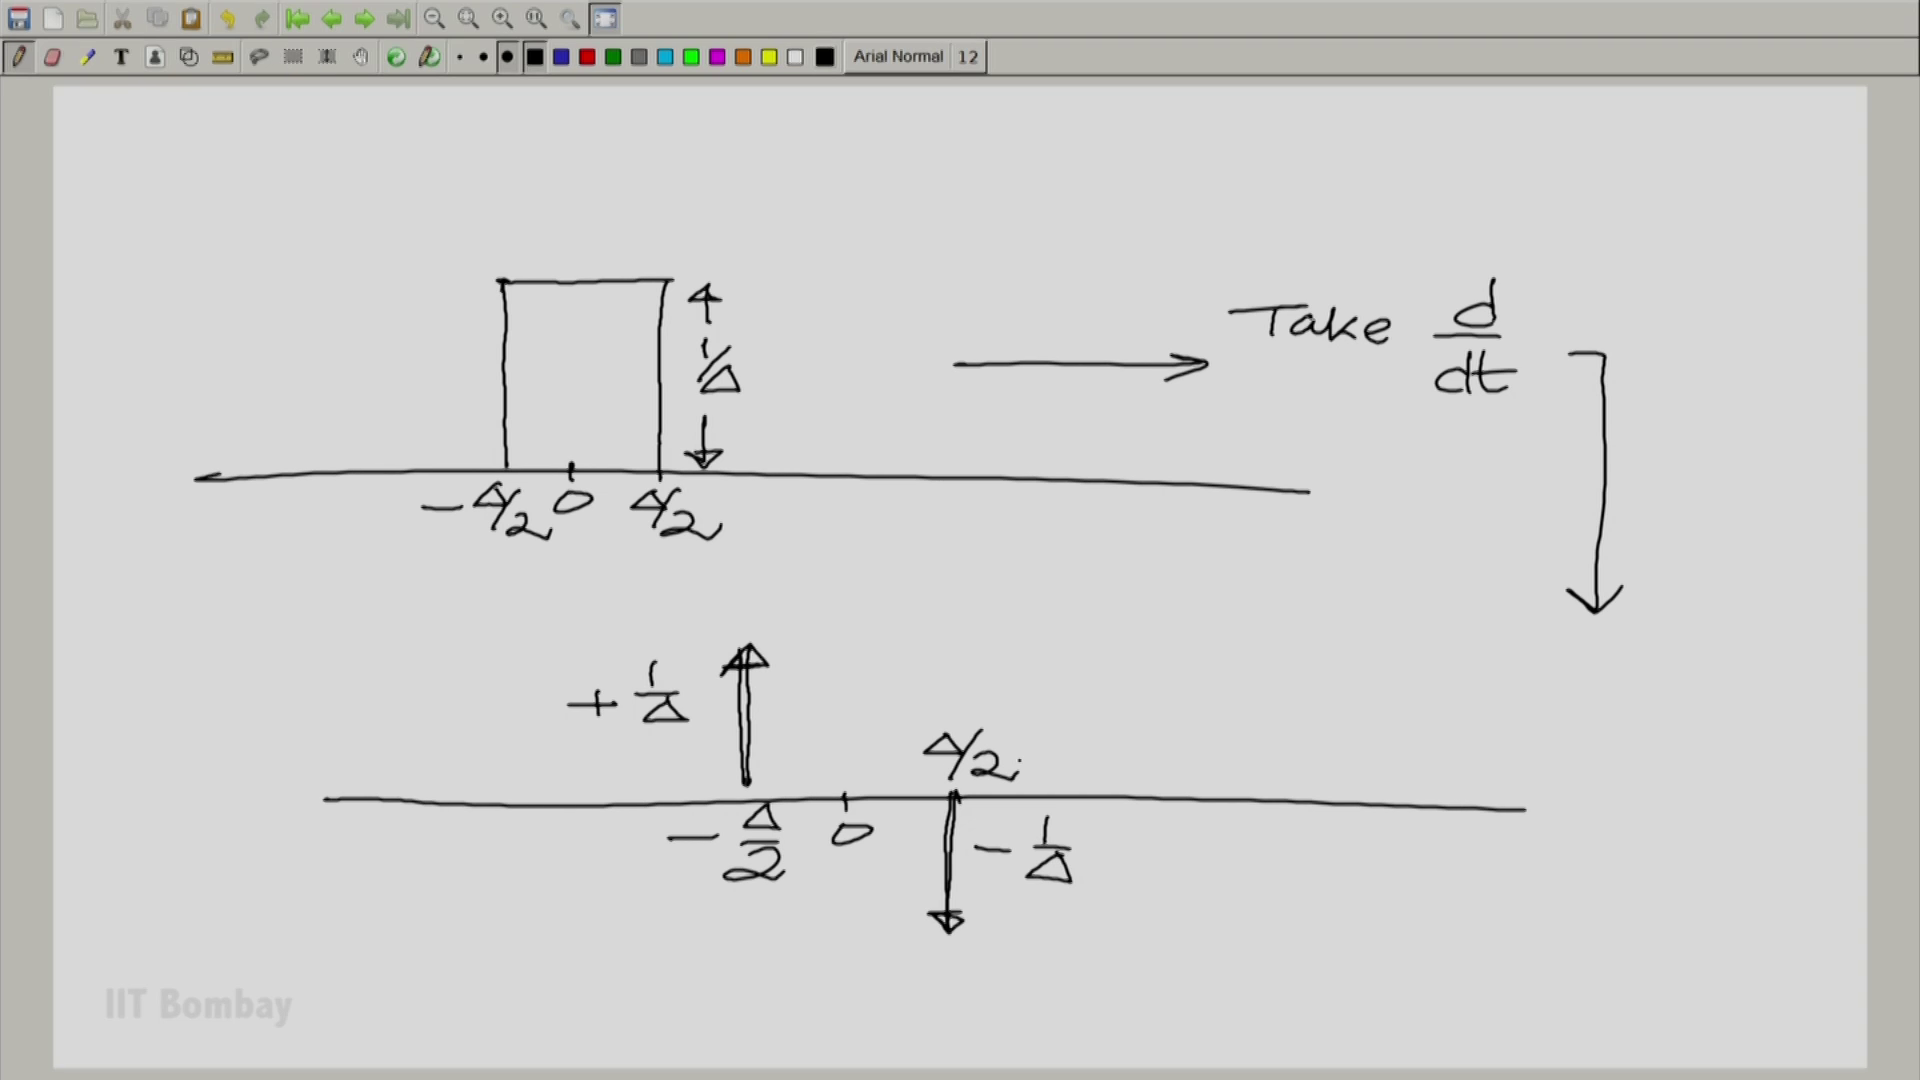
\includegraphics[width=10cm]{plot1.png}
\end{center}
\end{figure}

\noindent
In the above figure, the top one shows the impulse as $\Delta$ tends to zero and the bottom one is the derivative of the impulse. Now as $\Delta\rightarrow 0$, the impulse strength at $\frac{-\Delta}{2}\rightarrow \infty$ and $\frac{\Delta}{2}\rightarrow -\infty$ and these two come closer to each other. This is what we call as \emph{Doublet}. Suppose we let this doublet act upon a differentiable function $x(t)$ at point $t=t_0$.\\
\[
	 \int_{-\infty}^{\infty}{\frac{x(t)}{\Delta}(\delta(t-(t_0-\frac{\Delta}{2}))) - (\delta(t-(t_0+\frac{\Delta}{2})))} dt
\]
\noindent
which implies\\

\[
	\frac{x(t_0-\frac{\Delta}{2})-x(t_0+\frac{\Delta}{2})}{\Delta}
\]
\noindent
 As $\Delta$ tends to zero, the above expression will become the negative of the derivative of $x(t)$ at $t=t_0$. So we found by applying doublet over a differentiable function, we got the derivative of the function at that point. This doublet is usually called as \emph{Unit Doublet} as it is trying to be unit impulse as $\Delta\rightarrow 0$.\\
 
\noindent
We can extend this idea to find the inverse Laplace Transform of $s^2$. Here we need to do double differentiation of impulse, which implies differentiating the doublet. These generalised functions are called \emph{Singularity Functions}. It is easy to understand the effect of these impulses over functions rather than studying them in detail.\\

\subsection{RC Circuit}

\noindent
Now lets deal with the example of RC circuit. Let us find the unit step response using its Laplace Transform. Consider a RC circuit as shown in the below figure.\\
\begin{figure}[h!]
\begin{center}
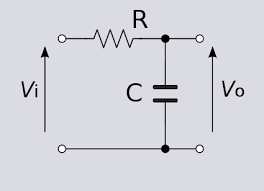
\includegraphics[width=5cm]{plot2.png}
\end{center}
\end{figure}

\noindent
Let the voltage across the resistor $R$ be $V_R(t)$ and the current passing through it be $i_R(t)$. We have\\
		\[ V_R(t) = i_R(t)R\]
        Taking Laplace Transform on both sides we get,
        \[ V_R(s) = i_R(s)R\]
        \[ \frac{V_R(s)}{i_R(s)} = R \]
        where R is known as Laplace domain Impedance of Resistance.
      
\noindent
Now consider the capacitor in the RC circuit. Let the voltage across the capacitor of capacitance $C$ be $V_c(t)$ and the current passing through it be $i_c(t)$.Then we have,\\
		\[  i_c(t) = C\frac{dV_c(t)}{dt}\]
        Taking Laplace Transform on both sides we get,
        \[  I_c(s) = CsV_c(s)\] 
        \[  \frac{V_c(s)}{I_c(s)} = \frac{1}{Cs}\]
        where $\frac{1}{Cs}$ is known as Laplace domain Impedance of Capacitance.
        
\noindent
Laplace domain Impedance with Laplace Transform will help to handle wide class of circuits consisting of resistances, inductors, capacitors etc.\\

\noindent
Consider the RC circuit. Let $V_i(t)$ be input voltage and $V_o(t)$ be the output voltage across capacitor. Then we have,
\[  V_i(t) = RC\frac{dV_o(t)}{dt} + V_o(t)\]
Taking Laplace Transform on both sides we get,
\[  V_i(s) = RCsV_o(s) + V_o(s)\]
\[  \frac{V_o(s)}{V_i(s)} = \frac{1}{1+RCs}\] 
Considering RC = $\tau$ (Time Constant),
\[  \frac{V_o(s)}{V_i(s)} = \frac{1}{1+s\tau}\] 
where $\frac{1}{1+s\tau}$ is known as system function. Now this system function has one pole at s = $\frac{-1}{\tau}$

\noindent
Since we have a single pole, there are two possible Region of Convergences(ROC). One is Right sided impulse response which has a region of convergence from ( $\frac{-1}{\tau}$,$\infty$). The other is the Left sided impulse response which has a region of convergence from (-$\infty$, $\frac{-1}{\tau}$). Considering the system to be causal, we need to consider only the Right sided impulse response which has a region of convergence from ( $\frac{-1}{\tau}$,$\infty$).\\

\noindent
In the RC circuit for the unit step input case, the Laplace Transform of unit step input is given by 
\[ u(t) \xrightarrow{\ \mathcal{L}\ } \int_{-\infty}^{\infty}{u(t)e^{-st}dt} = \int_{0}^{\infty}{e^{-st}dt} = \frac{1}{s} ; \enspace R_x = Re(s)>0 \]

\noindent
Therefore we have got $V_i(s)$ = $\frac{1}{s}$. Substituting this in the system function mentioned above, we get
\[  V_o(s) = \frac{1}{s(1+s\tau})\] 
\noindent
Expanding the above expression using partial fractions, we get\\
\[  V_o(s) = \frac{1}{s} - \frac{1}{s+\frac{1}{\tau}}\] 
\noindent
Here ROC will be the intersection of region of convergence of each terms. The first in the RHS of the above expression has a ROC of $Re(s) > 0$ while the other term has a ROC of $Re(s) > \frac{-1}{\tau}$. So taking intersection of these two ROC's, we get the final ROC which comes out to be $Re(s)>0$.\\

\noindent
Taking Inverse Laplace Transform on both sides we get,\\
\[  V_o(t) = u(t) - e^-(\frac{t}{\tau})u(t) = u(t)(1 - e^-(\frac{t}{\tau}))\]

\noindent
Clearly we can see that the above expression is indeed the step response of RC circuit which we had got earlier. Going ahead we can now calculate the response of a ramp input (a linearly increasing input) given by $V_i(t) = tu(t)$. The Laplace transform of $tu(t)$ comes out to be $\frac{1}{s^2}$. Now to calculate the ramp response we can follow two methods:\\

\begin{enumerate}
\item One is the above mentioned method i.e. calculate the partial fractions and perform inverse Laplace Transform on them.

\item The other is done by cascading the systems using running integrator. First a unit step input is given to RC Circuit and the output of RC circuit is given to the input of the running integrator. 

\end{enumerate}
\noindent
We can verify that in the both approaches we get the same answer.





























                



                     
